%%%%%%%%%%%%%%%%%%%%%%%%%%%%%% -*- Mode: Latex -*- %%%%%%%%%%%%%%%%%%%%%%%%%%%%
%% main.tex<fourier_decomp> -- 
%% Last Modified On: Thu Apr 13 16:15:17 2023 (+0200)
%%%%%%%%%%%%%%%%%%%%%%%%%%%%%%%%%%%%%%%%%%%%%%%%%%%%%%%%%%%%%%%%%%%%%%%%%%%%%%%

\documentclass{zamarep}

% Useful LaTeX packages
\usepackage{mathtools}
\usepackage{mathcalbd} % for \pol macro

\usepackage[colorlinks]{hyperref} % should be loaded last
\usepackage{cleveref}  % should be loaded last last

\title{Towards Verifiable TFHE}
\subtitle{Part 2: Proving Correct Execution of the Blind Rotation Using PLONK}

\author[MW]{Michael Walter}

% \date{April 13, 2023}

\titlegraphic[credit={Erik Karits}]{%
  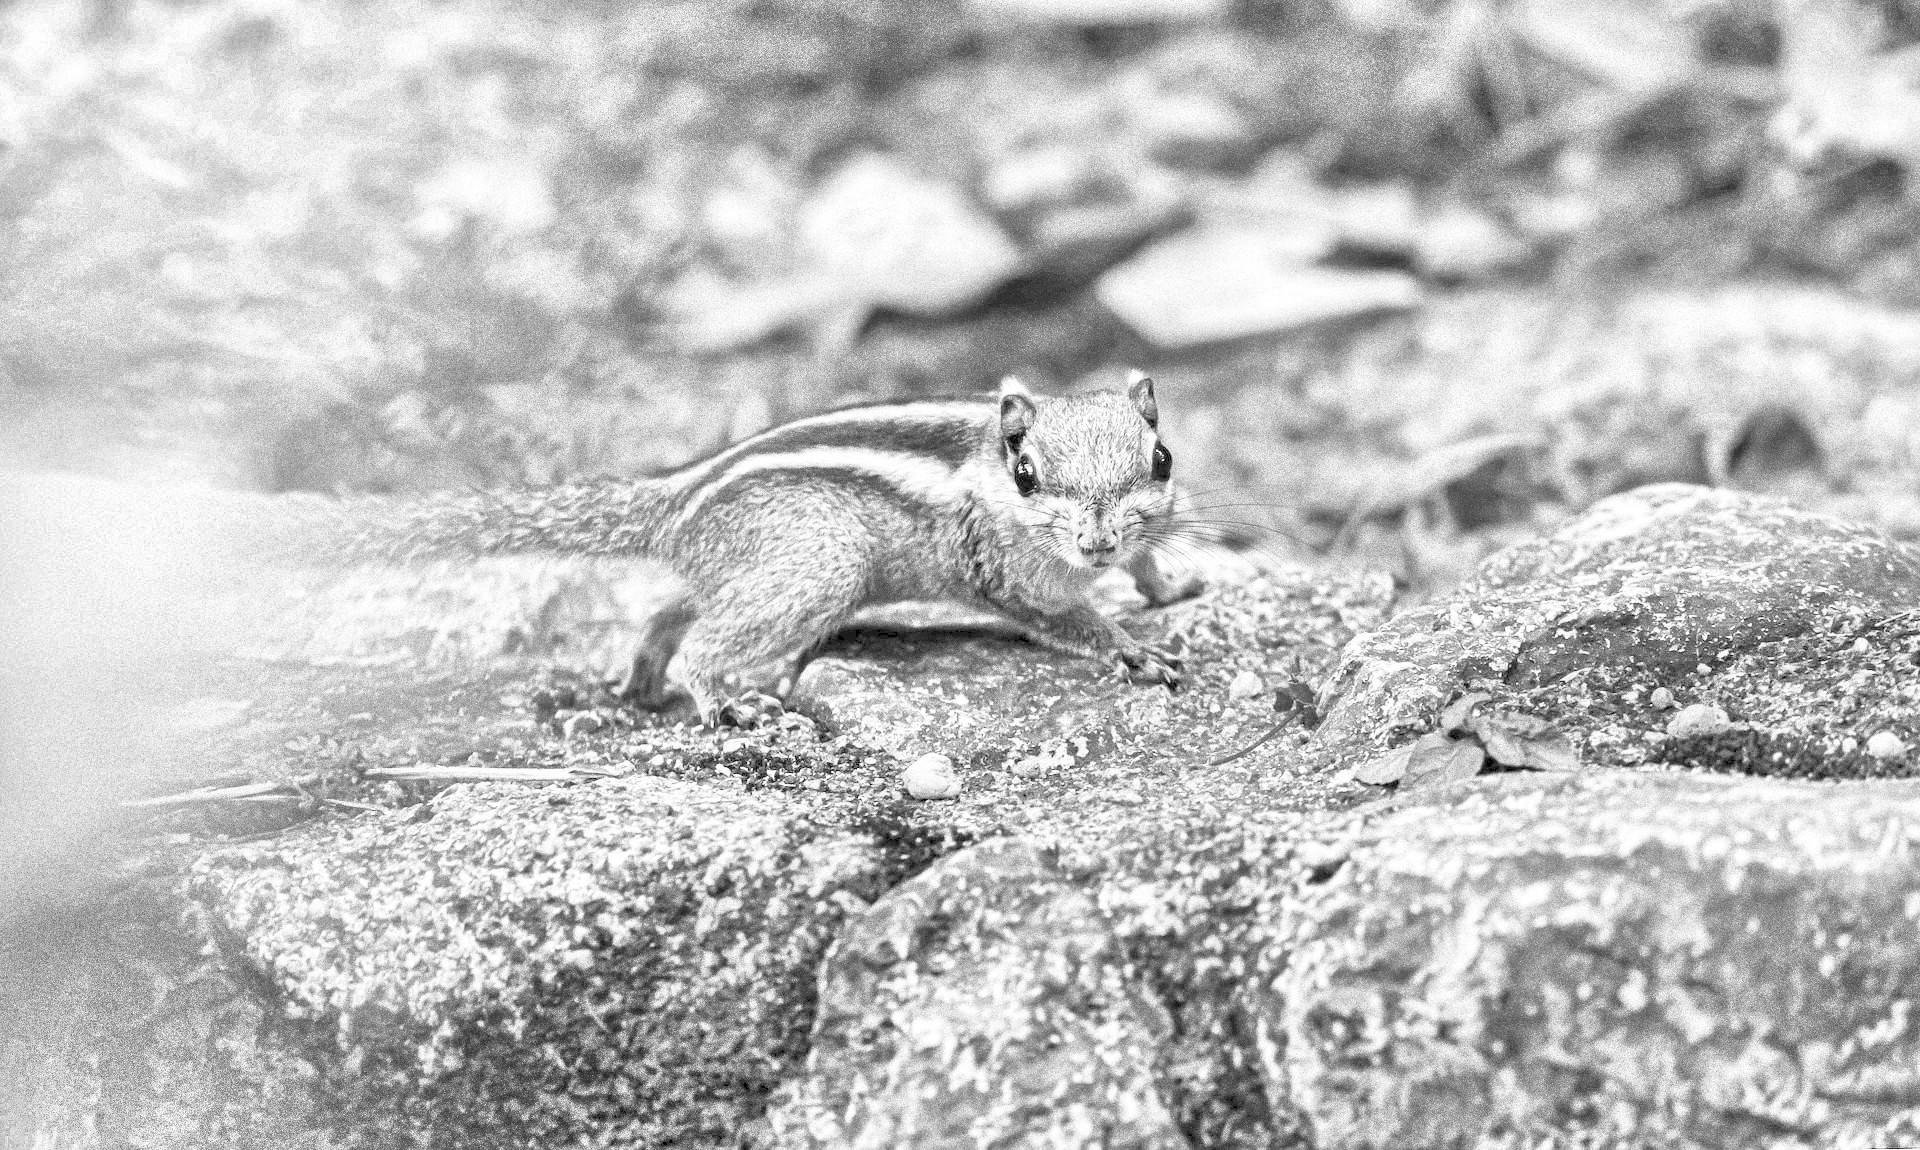
\includegraphics{erik-karits-Ivy_nqt6gTc-unsplash}}


% --- Macros
% \newcommand{\ints}{\mathds{Z}}
% \newcommand{\reals}{\mathds{R}}
% \newcommand{\torus}{\mathds{T}}
% \newcommand*{\pol}{\mathcalbd}
% \newcommand*{\SQ}{\mathit{S\!Q}}
\newcommand{\field}{\mathbb{F}}

\begin{document}

\maketitle


%%%%%%%%%%%%%%%%%%%%%%%%%%%%%%%%%%%%%%%%%%%%%%%%%%%%%%%%%%%%%%%%%%%%%%%%%%%%%%% 
\section{Introduction}\label{sec:introduction}
%%%%%%%%%%%%%%%%%%%%%%%%%%%%%%%%%%%%%%%%%%%%%%%%%%%%%%%%%%%%%%%%%%%%%%%%%%%%%%% 
This is part 2 of the documentation of our effort towards verifiable FHE. It describes improvements and extensions over the prototype presented in part 1 \cite{part1}. We attempted to keep this report as self-contained as possible, but it is more intelligible after reading part 1.

As outlined in part 1, our prototype consists of 3 parts: the polynomial commitment scheme (PCS) based on FRI \cite{ICALP:BBHR18}, the PLONK arithmetization \cite{EPRINT:GabWilCio19} and the code generating the circuits for FHE operations. We will describe the progress with respect to the three parts separately.

\section{Polynomial Commitment Scheme}
\label{sec:pcs}
Recall that the FRI based PCS involves using Merkle commitments to prove that a committed vector represents a low degree polynomial. More specifically, after committing to a polynomial $f$, this method shows that for $w = f(i)$ the polynomial $g(x) = (f(x) - w) / (x - i)$ is a low degree polynomial.

\subsection{Hash Function}
\label{sec:hash}
Since the PCS involves computing several Merkle commitments on large input vectors, the hash function is crucial for the performance of the entire SNARK. In part 1 we argued that an arithmetic hash function would be sensible, since it has the appeal of only having to deal with field elements, and we identified POSEIDON \cite{USENIX:GKRRS21} as a suitable candidate. But due to the lack of performant implementations easily callable from Sage, we decided to use SHA256 for now, converting to and from field elements when needed. (The hash output is converted by truncating and reducing modulus the field size.) When targeting a production ready implementation, the choice of hash function should be revisited as, e.g. POSEIDON can be implemented very efficiently and during a brief conversation the authors of \cite{USENIX:GKRRS21} offered their support. As outlined previously, an arithemtic hash function has the added benefit of allowing easier recursion should we choose to make use of that.

\subsection{Batch Openings}
\label{sec:batch}
In several places, we need to query the same committed polynomial at several points. The queries $i_j$ and their corresponding output values $w_j$ define the polynomials $g_j(x) = (f(x) - w_j) / (x - i_j)$, all of which we wish to prove to be low degree polynomials. An easy way to do so is to prove that $\sum_j \alpha^j g_j(x)$ is a low degree polynomial for a random challenge $\alpha$. Using this technique the complexity and proof size of many openings to the same polynomial is essentially the same as one opening.

\section{PLONK}
\label{sec:plonk}

The focus of the part 1 prototype was not on performance, so there were a lot of inefficiencies. This quarter, we performed a set of standard optimizations, like, e.g.,
\begin{itemize}
\item caching values instead of recomputing them,
\item performing more computations in the NTT domain,
\item computing lists of values more more efficiently,
\item breaking up the trace polynomial into 3 polynomials as in the original PLONK paper \cite{EPRINT:GabWilCio19}.
\end{itemize}
In sum, they yielded a significant performance improvement, but none of them are technically interesting enough to go into detail here.

\subsection{Lookup Arguments}
\label{sec:lookup}
Lookup arguments (see e.g., \cite{EPRINT:PFMBM22,EPRINT:GabWil20,halo2}) are a way for the prover to prove that some witness values are contained in a pre-defined table. (In fact, for some lookup arguments the table does not necessarily need to be pre-defined but can also be the result of a computation, but this is not important for us here.) We implemented the approach from \cite{halo2} in our prototype, using a selector polynomial to specify which values in the trace we require to be in the table. The lookup argument adds an overhead that is comparable to proving the correct wiring of the circuit, which is to be expected, since they use similar techniques.

\section{FHE Circuits}
\label{sec:circuits}

There are two main directions that the circuit generation developed: performance improvement (i.e. reducing the circuit size) and extension to blind rotation. Two main performance improvements were implemented: a) we use lookup arguments to prove that values resulting from the gadget decomposition are indeed small, and b) we implemented an NTT circuit, which we describe in the following. Both improvements allowed to drastically reduce the circuit size and thus prove circuits with larger parameters.

\subsection{Polynomial Multiplication via NTT}
\label{sec:ntt}

We replaced the naive multiplication method based on a matrix-vector product with an NTT based method. Specifically, we constructed a circuit for the Cooley-Tukey forward NTT and the Gentle\-man-Sande inverse NTT as described in \cite{EPRINT:LonNae16}. The external product requires $\ell$ forward NTTs and one inverse NTT, each requiring about $\frac32 N \log N$ gates, where $\ell$ is the decomposition parameter. So this is an improvement of $O(N /\log N)$ over the naive method.

\subsection{Approximate Decomposition}
\label{sec:decomp}

Our initial prototype only allowed for exact decomposition and used arithmetic gates for the range checks on the decomposed values. In contrast, we now use lookup arguments for the range checks and support approximate decomposition. Note though that even when using approximate decomposition, the values still need to be decomposed fully, but the lower order terms are ignored during the external product computation. The reason is that this approach implicitely performs a range check on the difference between the original value and the approximate decomposition. If we were to only compute the higher order terms of the decomposition, we would have to perform this check explicitely, likely through a decomposition again, which would yield the same complexity. We do note that the explicit check would add a degree of freedom: we could choose a different, maybe larger, base for this range check which could make it slightly more efficient.

\subsection{Blind Rotation}
\label{sec:blind}
Apart from simple polynomial additions, the only operation required for the blind rotation beyond the external product, is multiplication of a polynomial with a power of $X$. Specifically, on input a field element $a \in [0, 2 \cdot N)$ and a polynomial $p(X) \in \field_q[X]/(X^N + 1) $ (where we use standard Zama notation) represented by its coefficients, we wish to compute the coefficients of $X^a \cdot p(X)$. On a CPU this is trivial to do in $O(N)$, since it corresponds to a negacyclic rotation of the coefficients. If $a$ was fixed, this would be equally trivial for a circuit, since it would essentially just correspond to a rewiring of the input coefficients (plus a few negations). However, with $a$ being an input, this becomes significantly more involved for a circuit, since we cannot ``rewire'' a circuit at runtime.

We solved the issue by designing a circuit with $\log N$ layers of fixed rotations: for $1, 2, 4, 8 \dots N$ and a CMUX style circuit that selects either a rotated or the original polynomial depending on a control bit. Then we binary decompose $a$ and use the decomposition to perform the shift by $a$. Note that this approach requires $O(N \log N)$ gates and thus is of the order of an NTT computation.

\paragraph{Multiplication with negative powers of X}
There is another small caveat in the first step of the blind rotation. Here, we need to multiply the test vector with $X^{-b} $, where $b \in [0, 2\cdot N)$. This can be achieved by computing $\bar b = -b \mod 2N$ and then applying the circuit above. One might be tempted to simply compute $\bar b = 2N - b$, but unfortunately this does not quite work in case $b = 0$, since then $2N - b = 2N$ falls outside of the range $[0, 2N)$ and the binary decomposition will fail. We may extend the range of above circuit to $[0, 4N)$ by using another layer of fixed rotations, but then we would have to prove that $\bar b$ is in the range $[0, 2N]$ for correctness. (Note that the binary decomposition automatically does this check in the above case.) So instead we introduce a witness $w$ for $b$ that we enfore to be binary and then compute $2N \cdot w - b$. The prover then sets $w$ such that the result is in $[0, 2N)$ and applies the above circuit. Looking ahead, we remark  that this now might require an additional check that $b \in [0, 2\cdot N)$ after the modulus switch, once it is implemented, since a malicious prover could otherwise set $b$ to some negative value in $[-2N + 1, 0)$ and $w = 0$, which will not be detected by the verifier. Luckily, this does not significantly increase the circuit size, since this step only needs to be performed once. 

\subsection{Custom Gates for Polynomial Multiplication}
\label{sec:custom}
We explored an approach to use custom gates for polynomial multiplication in order to reduce the degree of the trace polynomials in the hope to improve efficiency. The main idea is to extend the trace to $3N$ columns, the first (second, third, resp.) $N$ representing the left input (right input, output, resp.) polynomial of a gate. The gates of the circuit would then have fan-in $2N$ and fan-out $N$ and would directly implement polynomial arithmetic. For large $N$, these gates are quite large, but the key observation here is that they have low-degree. So this did in fact significantly reduce the degree of the trace polynomial (asymptotically, by a $O(\log N)$ factor). Unfortunately, it overall resulted in an increased prover complexity, specifically for proving the correctness of the gates. Details follow.

On a very high level, when proving the correctness of the gate evaluations, the prover needs to compute each of the different gates once, but on degree-$d$ polynomials (where $d$ is roughly the circuit size). E.g. for simple (fan-in 2) multiplication, the prover needs to compute the polynomial $L(x) \cdot R(x)$. In a fan-in $2N$ multiplication gate, which implements multiplication in $\field_p[X]/(X^N + 1)$, the prover needs to compute a polynomial of the form
$$\sum_{j=0}^iL(\omega^{i-j}\cdot x) \cdot R(\omega^j \cdot x) - \sum_{j=i+1}^{N-1}L(\omega^{N-j+i}\cdot x) \cdot R(\omega^j \cdot x) $$
for all $i$. Even using Fast Fourier techniques, doing this naively costs $O(N^2 d)$ many operations. (Transform all $2N$ input polynomials to the NTT domain, compute the $ N^2$ products using component-wise multiplication, transform all $N$ output polynomial). A lot can be gained by selecting a suitable root of unity for the NTT transform and exploiting the structure of the polynomials (details can be found in the code), but still the fastest way we were able to compute these polynomials requires $O(N \cdot d)$ (which seems close to optimal, since there are $N \cdot d$ coefficients to compute). Since we think of $\log d \ll N$, prover time suffers when trading the $\log d$ factor for an $N$ factor, even if it reduces the degree $d$ by a factor $\log N$.

\section{Performance}
\label{sec:perf}
As in part 1, we assume TFHE to be parameterized with a prime ciphertext modulus $p$ such that we may match it with the field size of the SNARK and do not need to emulate arithmetic in a different ring. We let $n, N, k, \ell, B$ be the usual TFHE parameters. 

\subsection{Circuit Size}
\label{sec:csize}
To estimate the circuit size of a blind rotation, we focus on the parts with the dominant gate complexity: the NTT circuit and its inverse, and the multiplication with powers of $X$. The NTT circuit requires $\frac32 N \log N$ many gates, its inverse $\frac32 N \log N + N$. Ignoring the binary decomposition, the negacyclic rotation requires $N \log N$ CMUX gates -- $N$ for each layer -- and $N$ negations. Each CMUX gate is implemented as $(a_1 - a_0) \cdot b + a_0$ and thus requires 4 gates (one negation, one multiplication and two additions). So overall the rotation has size about $4 N \log N$. Ignoring lower order terms, we can estimate the circuit size of the blind rotation as $(k + 1) [4 (n + 1) +  \frac32 n (\ell + 1)]N \log N$. For realistic parameters like $N=1024$, $n=512$, $k=1$, $B=256$, and $\ell=2$ we get an (under-)estimate of about $2^{26}$ to $2^{27}$ gates. Recall that this corresponds roughly to the estimate of the external product in part 1, which means the improvements made this quarter reduced the circuit size by orders of magnitude.

\subsection{Performance and Proof Size for Small Instances}
\label{sec:small}
Here, we give some rough performance numbers for small instances. These numbers are mostly meant to give a sense of the concrete improvement w.r.t. the previous prototype. We stress that this is not a production ready implementation, neither with regards to security nor with regards to performance. We do note though that our parameters (and the choice of hash function, cf.\ Section \ref{sec:hash}) should provide roughly a \textasciitilde50 bit security level.

As an example, we choose the field size/ciphertext modulus to be $p=2^{64} - 2^{32} + 1$ and toy parameters $N=8$, $n=3$, $k=1$, $\ell=2$, and $B=256$. On the same hardware as in part 1, we are able to prove the correct execution of the blind rotation with these parameters in less than 30s. Verification takes about 2s and the proof consists of about 42k hash values and 11k field elements. This translates to roughly 1-2MB. The bulk of the proof is made up of hash values and we remark that using the full 256 bit output is somewhat of an overkill for a security level below 64 bits. We could truncate the hash output to 128bits halving the proof size. (Although it is questionable if this is useful, since eventually we will target a larger security level.)

The prototype scales very reasonably, e.g. if we increase the size of the LWE key to $n=6$, the prove requires about a minute to generate, verification take 4s and the proof size increases slightly to 48k hash values and 12k field elements, which is still less than 2MB.

As another point of comparison, we may prove a single step of the blind rotation with $N=32$, $k=1$, $\ell=2$, and $B=256$ in about a minute. This might be relevant if we are able to use IVC (see Section \ref{sec:ivc}) to prove the blind rotation.

\section{Outlook}
\label{sec:out}

\subsection{Refactoring}
\label{sec:refactor}

We believe, the code base is at a point where it would benefit significantly from a refactoring. With a better understanding of the system as a whole, we expect major improvements in readability and at least some improvements w.r.t. performance. For example, as outlined in Section \ref{sec:plonk}, we perform a lot of the polynomial arithmetic in the NTT domain, which means we need to perform NTT transforms on polynomials with relatively large degree. One target of the refactoring will be to minimize the number of transforms that need to be computed.

As outlined in Section \ref{sec:batch}, we may batch multiple PCS openings. The current code structure makes it difficult to take full advantage of this, as we separated the prover algorithm into different parts proving different properties of the trace polynomials. We hope to reduce the complexity for prover and verifier as well as the proof size by batching as many PCS openings as possible.

Recall that SNARKs require a preprocessing/setup that compresses some relevant information about the circuit for the verifier (so that it does not have to read the entire circuit). As pointed out in part 1, we currently assume that the prover performs the preprocessing (see part 1 for the justification), so we treat the preprocessing output as part of the proof. However, in many settings this is not justified and we plan to separate the preprocessing computation and output more cleanly from the core proof.

\subsection{Efficient Negacyclic Rotations Using Vector Lookups}
\label{sec:vector}
In Section \ref{sec:blind} we discussed that multiplication with $X^a$ in $\field_p[X]/(X^N + 1)$ are much more costly in a circuit than on a CPU. Here we describe an alternative approach based on polynomial multiplication. The lookup argument from \cite{halo2} can be extended to vector lookups, which means we can use it to prove that sets of witnesses appear as a row in a predefined multi-column table. This could be leveraged to map $a$ to the polynomial $X^a$ and then perform an NTT based multiplication with the other multiplicand. Clearly, we can map $a$ to the polynomial $X^a$ in the NTT domain directly, which saves one NTT transform. If we slightly change the blind rotation algorithm, we can improve on that: recall that during the blind rotation, we need to compute $X^a \cdot p - p$, where $p \in \field_p[X]/(X^N + 1)$. The result is decomposed and further processed during the external product. The first step of this further processing is to compute its NTT transform. We may be able to change the order in which the multiplication with $X^a$ and the decomposition are performed to reduce the number of required NTT transforms to $\ell$ (i.e.\ no additional NTT transforms): first decompose $p$ into the $\ell$ small polynomials, which are then transformed into the NTT domain, where we perform the rotation on all decomposed terms. Only then we perform the calculation of $X^a \cdot p - p$ on the decomposed terms. This works since decomposition is linear and would yield a complexity of $O(\ell N)$ for the negacyclic roation (plus the lookup argument).

There are two caveats to this approach: 1) If the decomposition is performed only approximately, the subtraction after decomposition doubles the error. We assume that this can be accommodated for by, e.g.\ adjusting the decomposition parameters $B$ and/or $\ell$, but this needs to be checked. 2) The length of the vector we need to map $a$ to is relatively large ($N$) and thus the table will have many columns. This comes at a price in the lookup argument of \cite{halo2}: each column requires a preprocessed polynomial and a PCS opening. For large $N$ this might become the dominant part of the proof size. However, we note that the columns of the table will be closely related as they will consist of powers of a root of unity. We expect that this structure can be used to reduce this overhead and hopefully obtain more efficient negacyclic rotation circuits.

\subsection{Custom Gates for Gadget Decomposition}
\label{sec:gadget}
Currently, in order to check the correctness of a gadget decomposition, we use a circuit that recombines the decomposed values and checks equality with the original value. This seems like an ideal use case for a custom gate, since it is a fixed operation that is performed very often. Unfortunately, it is not entirely straight-forward to include it, since this custom gate has a different fan-in ($\log_B p$) than the other gates (2). This is inconvenient, since the trace is typically encoded with a row for each gate and a column for each input/output wire. One could extend the number of columns to the maximum fan-in (+ output), but this would mean we ``waste'' a lot of space in the trace, which will result in inefficiencies in terms of running time and proof size. We plan to circumvent this problem by encoding a gate with larger fan-in using multiple rows.

\subsection{Incrementally Verifiable Computation}
\label{sec:ivc}

The blind rotation is essentially a loop where the same operation is repeated $n$ times with different input. There are some SNARKs that allow for recursion and/or folding, which allows to prove the individual loop steps separately and then fold them into one proof \cite{sangria,cryptoeprint:2023/620,TCC:Valiant08}. It is plausible that this will allow us to generate proofs for the blind rotation much more efficiently.

\subsection{Full PBS}
\label{sec:pbs}

There are three missing components to be able to prove a full PBS: 1) switching the modulus of an LWE ciphertext from $q$ to $2 \cdot N$, 2) the sample extraction, and 3) key switch. We plan to implement them in the near future, which will give us a sense of how large a circuit is required to prove the full PBS for realistic parameters.

% --- Bibliography
\bibliographystyle{alphaurl}
\bibliography{../../../cryptobib/abbrev1,../../../cryptobib/crypto,local}

\end{document}
